%!TEX root = informe.tex
\chapter{Metodología del Análisis de Ciclo de Vida}
\section{Introducción}

Como se ha mencionado en la sección \ref{sec:introantecedentes}, el Análisis de Ciclo de Vida de un producto incluye todos los procesos de producción y servicios relacionados con el producto durante su ciclo de vida completo, desde la extracción de las materias primas hasta su reciclaje y/o disposición final, pasando por la fabricación y los subproductos que lo forman, la instalación, el uso y mantenimiento del producto. También se pueden incluir en las diferentes etapas del ciclo de vida el almacenamiento, venta, transporte y otras actividades que se consideren relevantes.

El Análisis de Ciclo de Vida hace distinción entre ``Entradas'' —materias primas, energía— y ``Salidas'' —emisiones a la tierra, mar o aire, desechos y subproductos (figura \ref{fig:escenariolca}).

\begin{figure}[!htb]
\centering
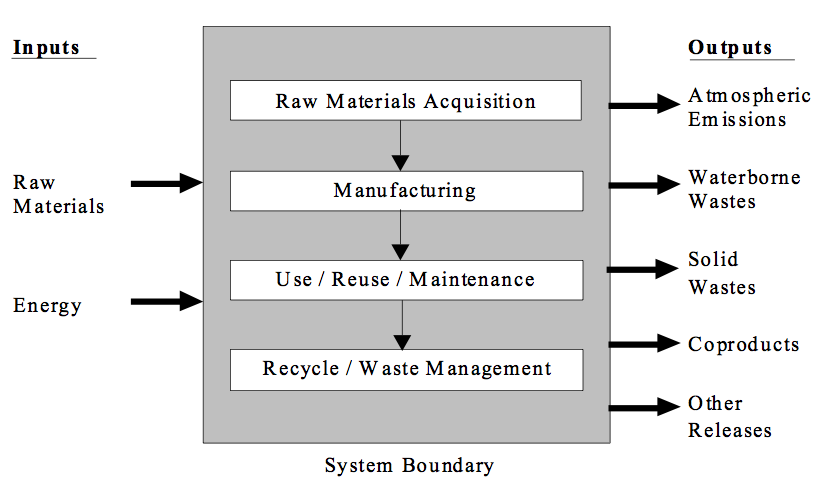
\includegraphics[width=12cm]{escenariolca.png}
\caption[Escenario de un ACV]{Escenario de un ACV. Fuente: basado en \protect\cite{epa}.}
\label{fig:escenariolca}
\end{figure}

En las ``Entradas'' también pueden aparecer productos que proceden de la \textbf{tecnoesfera} —productos no naturales—, que añadirán su historial medioambiental a los cálculos del producto y/o servicio. Para el caso de residuos, se tendrán que incluir los futuros procesos de tratamiento.

El Análisis de Impacto del Ciclo de Vida (AICV) recoge la totalidad de entradas y salidas a la naturaleza para realizar un estudio potencial de los efectos medioambientales relacionados con el producto \cite{iso14040}.

\subsection{Etapas del Análisis de Ciclo de Vida}

Según la norma UNE-EN-ISO 14040:2006, el estudio de Análisis de Ciclo de Vida se compone de cuatro fases, relacionadas según la figura \ref{fig:etapaslca}.

\begin{figure}[!htb]
\centering
\includegraphics[width=12cm]{etapaslca.png}
\caption[Etapas del Análisis de Ciclo de Vida.]{Etapas del Análisis de Ciclo de Vida. Fuente: \protect\cite{iso14040}.}
\label{fig:etapaslca}
\end{figure}

\subsubsection{Fase de definición de objetivos y alcance}
En esta fase se define el objetivo y el uso previsto del estudio, al mismo tiempo que el alcance de acuerdo con los límites del sistema, la unidad funcional y los flujos dentro del ciclo de vida, la calidad exigida a los datos, y los parámetros tecnológicos y de evaluación \cite{iso14040,ihobeeco}.

\subsubsection{Fase de Análisis de Inventario (ICV)}
En esta fase se recogen los datos correspondientes a las entradas y salidas para todos los procesos del sistema de producto. Es necesario definir el ciclo de vida del producto

\subsubsection{Fase de Evaluación del Impacto Ambiental (EICV)}
Es la fase del ACV en la que el inventario de entradas y salidas es traspasado a indicadores de potenciales impactos ambientales al medio ambiente, a la salud humana y a la disponibilidad de recursos naturales.

\subsubsection{Fase interpretación}
Es la fase del ACV en la que los resultados del ICV y el EICV son interpretados de acuerdo al objetivo y alcance marcados inicialmente. En esta fase se realiza un análisis de los resultados y se marcan las conclusiones.

\subsection{Ventajas e inconvenientes del ACV}

El Análisis de Ciclo de Vida es una herramienta que ofrece muchas ventajas:
\begin{itemize}
  \item el ACV es la única herramienta que examina los impactos medioambientales de un producto y/o servicio a través de su ciclo de vida.
  \item el ACV es un método estándar ISO, en referencia a las normas ISO 14040 e ISO 14044.
  \item el ACV proporciona una visualización fácil de entender de separando en etapas las fuentes de impacto.
  \item el ACV puede tanto guiar las decisiones de un fabricante (nivel microeconómico) como ayudar a un gobierno a definir una política de actuación (nivel macroeconómico).
  \item el ACV distingue entre la información relevante mediante cuantificación objetiva y los asuntos que pertenecen a políticas y elecciones sociales.
\end{itemize}

Por otro lado, el Análisis de Ciclo de Vida tiene ciertas limitaciones:
\begin{itemize}
  \item los resultados son geográficamente dependientes. Los resultados de un estudio en Europa no son aplicable en Estados Unidos sin tener en cuenta las variaciones geográficas correspondientes (por ejemplo, el mix eléctrico).
  \item el ACV sólo evalúa los impactos potenciales, no los verdaderos impactos, por lo que no proporciona ninguna información de las consecuencias.
  \item los resultados de dos ACVs para un mismo objeto de estudio puede diferir según los objetivos, procesos, calidad de los datos y el método de análisis de impacto utilizados. La ISO insiste en transparencia a la hora de realizar un ACV.
  \item un ACV detallado requiere un inventario de todos los procesos elementales incluidos dentro de los parámetros del sistema.
  \item se requiere el uso de bases de datos, software especializado y personas capacitadas para poder analizar los datos.
\end{itemize}

\section{Métodos de análisis de aspectos ambientales de productos y establecimiento de prioridades}

Existen varios métodos —cualitativos y cuantitativos— para analizar el perfil ambiental de un producto y establecer prioridades ambientales. Todos ellos se basan en el Análisis del Ciclo de Vida, lo que significa que analizan todas las fases del ciclo de vida del producto en cuanto a los aspectos ambientales del producto en cada una.

Los objetivos de estos métodos son:
\begin{itemize}
  \item Obtener una perspectiva general de los principales aspectos ambientales del producto durante todo su Ciclo de Vida.
  \item Identificar las prioridades ambientales.
\end{itemize}

A continuación se analizarán brevemente algunos de los métodos más interesantes: Matriz MET, Eco-indicadores y el software de Análisis de Ciclo de Vida. Éste último, debido a su importancia actual y a que son el método utilizado en este proyecto, será desarrollado con mayor amplitud en la sección \ref{sec:software}.

\subsection{Matriz MET}

La Matriz MET (Materiales/Energía/Toxinas) es una método cuantitativo y cualitativo con el que se obtiene una visión global de las entrada y salidas de cada etapa del Ciclo de Vida del producto. Es cuantitivo porque maneja cantidades, pero también se trata de un método cualitativo porque prioriza los aspectos ambientales y se basa en conocimientos ambientales y reglas de oro y no en cifras o resultados \cite{ihobeeco}.

La Matriz MET engloba:
\begin{itemize}
  \item M: utilización de Materiales en cada etapa del ciclo de vida. Incluye todas las entradas (consumos) de cada una de las etapas del ciclo de vida, proporcionando una visión de cuáles son las prioritarias por su mayor cantidad, toxicidad o por ser materiales escasos.
  \item E: utilización de Energía. Engloba el impacto de los procesos y transportes en cada una de las etapas del ciclo de vida —principalmente aquellos que consumen mucha energía—, proporcionando una visión de cuáles son los procesos o transportes de mayor impacto.
  \item T: emisiones Tóxicas. Recoge todas las salidas producidas en el proceso —emisiones, vertidos o residuos tóxicos—, proporcionando las salidas más importantes por su toxicidad.
\end{itemize}

El uso de la Matriz MET se recomienda:
\begin{itemize}
  \item Para recopilar datos antes de utilizar los Eco-indicadores o software de Análisis de Ciclo de Vida, ya que permite organizar la información de cada etapa del ciclo de vida.
  \item Para obtener una visión global rápida de las prioridades ambientales sin la necesidad de gran precisión.
  \item Como método alternativo cuando no existan Eco-indicadores relevantes para los materiales o los procesos del producto.
\end{itemize}

\subsection{Eco-indicadores}

El Eco-indicador es una método cuantitativa de fácil manejo. Es más preciso que la Matriz MET a la hora de priorizar los principales aspectos ambientales del producto en su ciclo de vida. Es un método cuantitativo porque la priorización se basa en cálculos numéricos \cite{ihobeeco}.

Los Eco-indicadores son el resultado de un proyecto desarrollado por un equipo multidisciplinar formado por industrias punteras de diferentes sectores, científicos de centros de investigación independientes y el gobierno holandés con el objetivo de intentar conseguir evaluar el impacto ambiental que ejerce la actividad industrial sobre el medio ambiente, centrándose en el impacto sobre el ecosistema, los recursos y la salud humana a nivel europeo. Los impactos tenidos en cuenta son: el efecto invernadero, la reducción de la capa de ozono, la lluvia ácida, la disminución de los recursos naturales, la disminución de la biodiversidad y el smog fotoquímico.

Existen diversos métodos basados en Eco-indicadores, entre los que cabe destacar \cite{mlgceballos}:

\begin{itemize}
  \item CML 2001: desarrollado en los Países Bajos, basado en su versión de 1992. El paso de normalización es opcional para ACVs simplificados, pero obligatorio para los exhaustivos. Las categorías de impacto ambiental son: agotamiento de los recursos abióticos, cambio climático, destrucción de capa de ozono, toxicidad humana, ecotoxicidad, smog fotoquímico, acidificación, eutrofización y uso de recursos.
  \item ReCiPe: del mismo equipo que la metodología EICV (ver sección \ref{sec:recipe}). Las categorías de impacto ambiental son: destrucción de capa de ozono, toxicidad humana, radiación, smog fotoquímico, formación de partículas, cambio climático, ecotoxicidad del suelo, acidificación del suelo, ocupación del suelo rural, ocupación de suelo urbano, transformación suelo natural, ecotoxicidad marina, eutrofización marina y agua dulce, ecotoxicidad de agua dulce.
  \item Ecoindicator 95: desarrollado por PRè Consultants, se basa en la existencia de una correlación entre la gravedad del efecto produccido por las emisiones y la distancia entre el nivel actual de emisiones y un nivel objetivo marcado como estándar de calidad ambiental, según un modelo de distancias al nivel objetivo.
  \item Ecoindicator 99: considera tres categorías de daños, relacionadas directamente con el resultado del inventario: salud humana, calidad del ecosistema y agotamiento de recursos. El Ecoindicador 95 es más un indicador de emisiones mientras que el Ecoindicador 99 lo es más de combustibles fósiles.
  \item EcoPoint: desarrollado por el Ministerio de Medioambiente de Suiza (BUWAL) en 1990, actualizado en 1997. Se basa en la distancia al objetivo que ofrece como resultado un indicador de impacto único.
  \item EPS: desarrollado por el Instituto de Investigación Medioambiental de Suecia en 1991. Se basa en una valoración de economía ambiental, es decir, determinar el daño y su asignación monetaria, en unidades ELU (Environmental Load Unit).
\end{itemize}

\section{Software de Análisis de Ciclo de Vida}\label{sec:software}

El mercado ofrece una amplia gama de programas para el Análisis de Ciclo de Vida que ofrecen diferentes tipos de prestaciones y rangos de precios. Entre ellos cabe destacar:

\begin{itemize}
  \item SimaPro: ver sección \ref{sec:simapro}.
  \item Gabi: permite esbozar ideas en su interfaz y ofrece un potente asistencia para la creación del inventario. Incorpora una base de datos propietaria que también funciona con \textit{ecoinvent}. Es compatible con los estándares ISO 14040 y bastante flexible.
  \item Quantis Suite: facilita el acceso a personas no expertas con plantillas y asistentes. Incorpora una base de datos propia.
  \item EarthSmart: permite crear inventarios de forma rápida aunque el usuario no sea experto. Permite crear un final de vida basado en escenarios creados por expertos. Incorpora varias bases de datos como \textit{ecoinvent} y la Australian LCI database.
  \item Eco-it: desarrollada para la Sociedad Pública de Gestión Ambiental del País Vasco (IHOBE). Realiza Análisis de Ciclo de Vida simplificado basado en la metodología ReCiPe, así como Huella de Carbono basado en valores IPCC. Es compatible con la normativa ISO 14040.
  \item openLCA: es una aplicación profesional de código abierto y gratuita para Análisis de Ciclo de Vida y Huella de Carbono creada por GreenDelta.
\end{itemize}

El paquete de software utilizado para este proyecto será SimaPro debido a la versatilidad que aporta, disponibilidad, inclusión de base de datos \textit{ecoinvent} y su compatibilidad con la norma ISO 14040.

\subsection{SimaPro}\label{sec:simapro}
SimaPro es una herramienta profesional desarrollada por la empresa holandesa PRé Consultants para el Análisis de Ciclo de Vida más utilizada actualmente por la mayor parte de los consultores y la industria, apoyada en la investigación de materiales y elementos por parte institutos y universidades \cite{mgoedkoop}. Permite modelar ciclos de vida complejos y analizarlos de forma sistemática y transparente, ya que puede rastrearse el origen de todos los resultados de forma sencilla.

\begin{figure}[!htb]
\centering
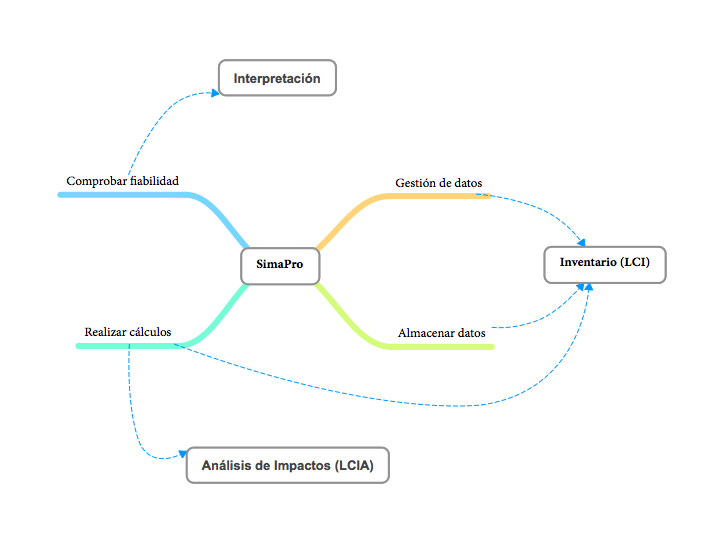
\includegraphics[width=13cm]{simapro.png}
\caption{Estructura de SimaPro.}
\label{fig:simapro}
\end{figure}

Entre sus principales cualidades destacan:

\begin{itemize}
  \item Diseño de productos.
  \item Desarrollo de indicadores clave.
  \item Cálculo de la huella de carbono de muchos tipos de productos y sistemas.
  \item Determinar el impacto medioambiental de productos o servicios con precisión estadística mediante el método de análisis Monte Carlo.
  \item Incluye Declaraciones Medioambientales de Productos e Informes Medioambientales GRI (Global Reporting Initiative).
  \item Utilización de bases de datos con inventarios.
  \item Asignación de múltiples procesos de salida.
  \item Análisis de Punto Débil, que permite identifica los puntos sensibles en el ciclo de vida utilizando un árbol de procesos.
  \item Análisis de tratamientos de residuos y escenarios de reciclado.
\end{itemize}

Esta herramienta cuenta con una interfaz de usuario intuitiva con un explorador de guía a través del Análisis de Ciclo de Vida del producto o servicio siguiendo los principios de las normas ISO 14040 y 14044. Además incorpora un modelado utilizando un asistente paso a paso.

La mayor ventaja de esta herramienta es la utilización de bases de datos con los inventarios de miles de procesos y métodos más importante de análisis de impacto.

SimaPro incluye varias bases de datos de inventarios con miles de procesos, además de los métodos de análisis de impacto más importantes. De esta forma, no es necesario recolectar datos de procesos individuales y poder centrarse en los asuntos más importantes del estudio.

\begin{figure}[!htb]
\centering
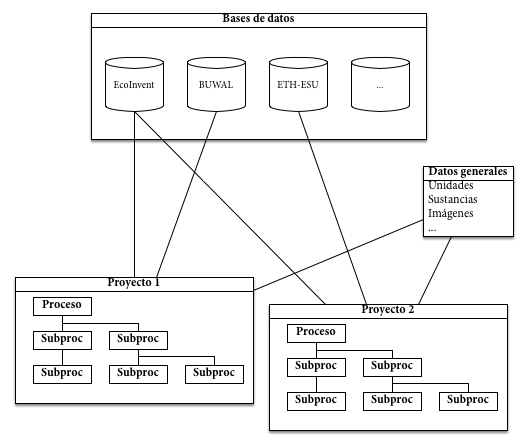
\includegraphics[width=15cm]{bbddsimapro.png}
\caption{Estructura de una base de datos de SimaPro.}
\label{fig:bbddsimapro}
\end{figure}

\section{Bases de datos}

La calidad de los datos que aparecen en el Inventario de Ciclo de Vida (ICV) tienen gran importancia en la relevancia del estudio que se realice. En función de la base de datos utilizada el Análisis de Ciclo de Vida puede obtener resultados diferentes.

La metodología de uso del software de Análisis de Ciclo de Vida consiste en utilizar una base de datos como soporte para aquellos materiales y procesos de nuestro sistema que sean similares con los de la base de datos. En caso de que no se adapten a la entrada de la base de datos será necesario modelar una nueva entrada equivalente, pudiendo usar otras entradas de la base de datos.

Cuando se habla de bases de datos (BBDD) en el marco de un ACV, se pueden diferenciar, en función de los datos que contengan, dos tipos:
\begin{itemize}
  \item BBDD con las entradas/salidas que se emplean para simular el sistema analizado en el Inventario de Ciclo de Vida (ICV), conocidas como BBDD de ICV.
  \item BBDD con los datos que cada metodología de Evaluación de Impacto del Ciclo de Vida (EICV) necesita para que la herramienta que llevará a cabo el EICV haga los calculos, conocidas como BBDD de metodologías.
\end{itemize}

Las bases de datos de Inventarios de Ciclo de Vida (ICVs) están formadas por datos de muy diversos materiales y procesos, normalmente agrupados según la fase del ciclo de vida a la que hagan referencia. A través de ellas se puede asignar a cada entrada/salida reflejadas en el ICV una serie de información de la base de datos que indicará la información sobre su impacto ambiental, los factores de caracterización, normalización, etc \cite{ihobecarbono}.

Las bases de datos de metodologías están formadas por los factores de caracterización, ponderación y otros datos que cada metodología de EICV necesita para realizar los cálculos de obtención de resultados. Estas bases de datos recogen los datos en un formato estándar y común (ISO/TS 14048:2002), para que el software de Análisis de Ciclo de Vida pueden utilizar estos datos \cite{ihobecarbono}.

SimaPro (ver sección \ref{sec:simapro}) incorpora varias bases de datos de Inventarios de Ciclo de Vida:
\begin{itemize}
  \item ecoinvent (2009): más de 4000 procesos en energía, transporte, materiales; incluye construcción, químicos, agricultura, etc.; unidad y procesos de sistema.
  \item BUWAL 250 (1997): materiales generales, energía, transporte y desechos, parcialmente basada en base de datos ETH.
  \item ETH-ESU (1996): reconocida base de datos de energía y transporte.
  \item USA Input Output (2003): datos Entrada/Salida para los EE.UU.
  \item Industry data (2001): datos publicados por asociaciones industriales, como APME.
  \item Idemat (2001): base de datos holandesa, recopilada de diferentes fuentes.
  \item Franklin (1996): base de datos generales de EE.UU. sobre materiales, transporte y energía.
  \item Danish IO y Danish Food (2003): bases de datos de Dinamarca de Entrada/Salida y comida.
\end{itemize}

Entre las bases de datos de metodologías de Evaluación de Impactos de Ciclo de Vida, SimaPro incorpora las siguientes:
\begin{itemize}
  \item Efecto 2002: estimación de daños; muchas similitudes con Eco-indicador 99, pero con factores de toxicidad recalculados.
  \item TRACI 2002: método Midpoint desarrollado por US EPA.
  \item CML 2 baseline 2000: actualización del método de 1992, modelos re- avanzados e inclusión de análisis de destino.
  \item EPS 2000: Estimación de daños, usando monetarización (intención de pagar) en lugar de peso por un panel. No hay necesidad de normalización en esta estimación.
  \item Eco-indicator 99: estimación de daños; usa indicadores de categoría en el nivel final. Se incluyen tres versiones usando diferentes suposiciones en los modelos medioambientales.
  \item Ecopoints 97 (UBP): distancia al objetivo basado en objetivos de políticas suizas (conocido también como método de escasez o UBP).
  \item EDIP 97: método de caracterización y normalización desarrollado por EPA de Dinamarca.
  \item Eco-indicator 95: distancia al método objeto basado en objetivos científicos e incluye estimación de daños.
  \item CML 92: método “midpoint” (punto intermedio) bastante usado, caracterización relativamente simple, sin destino o exposición, varios sets de normalización.
\end{itemize}

\subsection{ecoinvent}\label{sec:ecoinvent}

\textit{ecoinvent} implementa en una única base de datos miles de conjuntos de datos de ICVs —agricultura, energía, transporte, combustibles, biomateriales, químicos, materiales de construcción, materiales de empaquetamiento, metales elementales y preciosos, procesado de metales, informática y electrónica, tratamiento de residuos— basados en información industrial recopilada por grupos de investigación y consultores reconocidos internacionalmente \cite{website:ecoinvent}.

\begin{figure}[!htb]
\centering
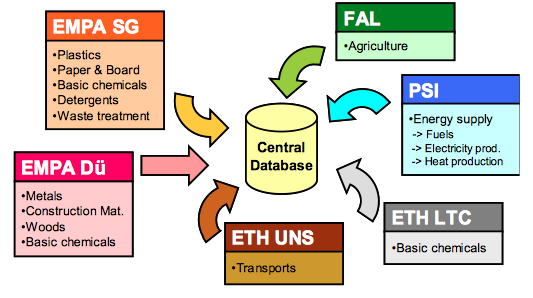
\includegraphics[width=13cm]{bbddecoinvent.png}
\caption[Estructura de la base de datos de \textit{ecoinvent}.]{Estructura de la base de datos de \textit{ecoinvent}. Fuente: \protect\cite{mgoedkoop2}.}
\label{fig:bbddecoinvent}
\end{figure}

La base de datos \textit{ecoinvent}:
\begin{itemize}
  \item Incorpora más de 4000 procesos:
  \begin{itemize}
    \item Bienes de producción y calidades.
    \item Para algunos procesos añade diferencias regionales (Suiza y Unión Europea).
    \item Mix eléctrico y procesos agrícolas de Estados Unidos y Asia.
  \end{itemize}
  \item Incertidumbre en los datos.
  \item Ilustraciones de la mayoría de los procesos.
  \item Documentación extensa y consistente de los procesos.
  \item Actualizaciones frecuentes y periódicas.
  \item Incluye versiones de los procesos como Unidad (Proceso 1/U) —más detallado— o como Sistema (Proceso 1/S) —sin información de incertidumbre—.
\end{itemize}

\section{Metodología para Evaluación del Impacto del Ciclo de Vida}

La base de datos \textit{ecoinvent} ofrece múltiples métodos para la evaluación de impactos que aplican diferentes factores —caracterización, normalización, peso y daño— a cada flujo elemental de la tabla de inventario según su implementación. Los métodos más destacables que se tendrán en cuenta en este proyecto son:

\begin{itemize}
  \item Método ReCiPe: categorías de impacto y áreas de protección del medio ambiente.
  \item Método de Demanda de Energía Acumulada: cuantificación de energía consumida.
  \item Método IPCC 2007: cálculo potencial del calentamiento global a lo largo del ciclo de vida.
\end{itemize}

\subsection{ReCiPe}\label{sec:recipe}

El desarrollo de ReCiPe se debió al principio a integrar la metodología orientada al problema de \textit{CML-IA} y la metodología orientada al daño de \textit{Ecoindicator 99}. De esta manera, ReCiPe se convirtió en el sucesor de ambos métodos \cite{mgoedkoop3}.

La metodología orientada al problema de \textit{CML-IA} define las categorías de impacto en el punto medio. La incertidumbre de los resultado en este punto es relativamente baja. El inconveniente de este sistema es la ambigüedad de las conclusiones al haber demasiadas categorías de impacto.

La metogología orientada al daño de \textit{Ecoindicator 99} aborda sólo tres categorías de impacto, lo que hacer más fácil obtener conclusiones. Sin embargo, la incertidumbre de los resultados es más alta que con la otra metodología.

ReCiPe implemente ambas estrategias incluyendo las categorías de impacto tanto a punto medio como a punto final. A los factores de caracterización a punto medio se les aplica un factor de daño para obtener los valores de caracterización de punto final. ReCiPe comprende un total de 21 categorías de impacto agrupadas en 2 conjuntos (ver figura ref{recipecategoriasimpacto}):
\begin{itemize}
\item Punto medio: 18 categorías de impacto.
\item Punto final: 3 categorías de impacto.
\end{itemize}

\begin{figure}[!htb]
\centering
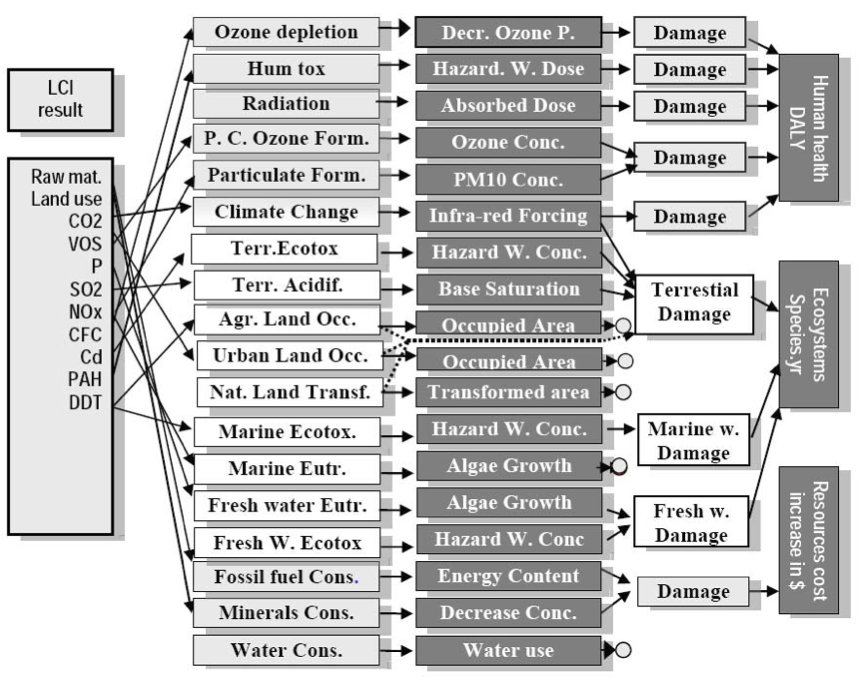
\includegraphics[width=12cm]{recipecategoriasimpacto.png}
\caption[Categorías de impacto aplicadas por ReCiPe.]{Categorías de impacto aplicadas por ReCiPe. Fuente: \protect\cite{mgoedkoop3}.}
\label{fig:recipecategoriasimpacto}
\end{figure}

\subsection{Demanda de Energía Acumulada}

Esta metodología —desarrollada a principio de los 70 debido a la crisis del petróleo— permite investigar el uso de energía a través del ciclo de vida de un producto o servicio. El análisis de la Demanda Acumulada de Energía consiste en la cuantificación tanto del uso directo como directo de energía —o consumo gris— durante todo el ciclo de vida del producto \cite{ecoinventlcia}.

Los valores CED (Cumulate Energy Demand) pueden utilizarse para comparar los resultado de un estudio detallada de Análisis de Ciclo de Vida con otros donde se indica únicamente la demanda de energía. También pueden utilizarse como indicador de verificación de los datos ya que es bastante fácil juzgar en base a la Demanda de Energía Acumulada si se han cometido errores importantes o no \cite{ecoinventlcia}.

Debido a que existe divergencias en los conceptos para la caracterización de las fuentes de energía primarias, los indicadores CED se dividen en ocho subcategorías para su uso con la base \textit{ecoinvent}, divididos en dos categorías base:

\begin{itemize}
  \item Fuentes no renovables: fósil, nuclear y bosque primario.
  \item Fuentes renovables: biomasa, viento, solar, geotérmica y agua.
\end{itemize}

\subsection{IPCC 2007}

El método IPCC 2007 —Intergovernmental Panel on Climate Change— es una actualización su homónimo de 2001. Este método es uno de los más empleados en la evaluación de impactos ya que realiza una caracterización de diferentes emisiones gaseosas de acuerdo a su Potencial de Calentamiento Global —Global Warming Potencial, GWP— y al conjunto de diferentes emisiones en la categoría de impacto de calentamiento global. Los valores de caracterización para las emisiones de gases de efecto invernadero se basan en los potenciales de calentamiento global publicados por el propio Grupo Intergubernamental de Expertos sobre el Cambio Climático (IPCC).

Al igual que en la versión de 2001, se establecen tres horizontes temporales para mostrar los efectos de la duración en la atmósfera de los diferentes gases:

\begin{itemize}
  \item GWP 20a (20 años).
  \item GWP 100a (100 años).
  \item GWP 500a (500 años).
\end{itemize}

Los Potenciales de Calentamiento Global (GWPs) directos están relacionados con el impacto del dióxido de carbono (\ce{CO2}). Los GWPs son un índice para la estimación de la contribución de calentamiento global relativo debido a las emisión atmosférica de un kilogramo de un gas de efecto invernadero concreto comparado con la emisión de un kilogramo de \ce{CO2} \cite{ecoinventlcia}.
